\documentclass{beamer}
\usepackage{times, amsthm, amsmath, amssymb, cancel, changepage, graphicx, lipsum, fancyhdr, mathabx, enumitem,caption, subcaption}
\usetheme{CambridgeUS}
\usecolortheme{seagull}
\usefonttheme{serif}
\definecolor{navy}{RGB}{0, 0, 128} 
\setbeamercolor{frametitle}{fg=navy}
\setbeamercolor{title}{fg=navy}

\title{Lecture 9: Multiple Integration Part I}
\date{September 24, 2019}

\begin{document}
	
\frame{\titlepage}

\begin{frame}
\frametitle{\textbf{Single to Double Integration}}
\begin{figure}
	\centering
	\begin{subfigure}{0.48\textwidth}
		
		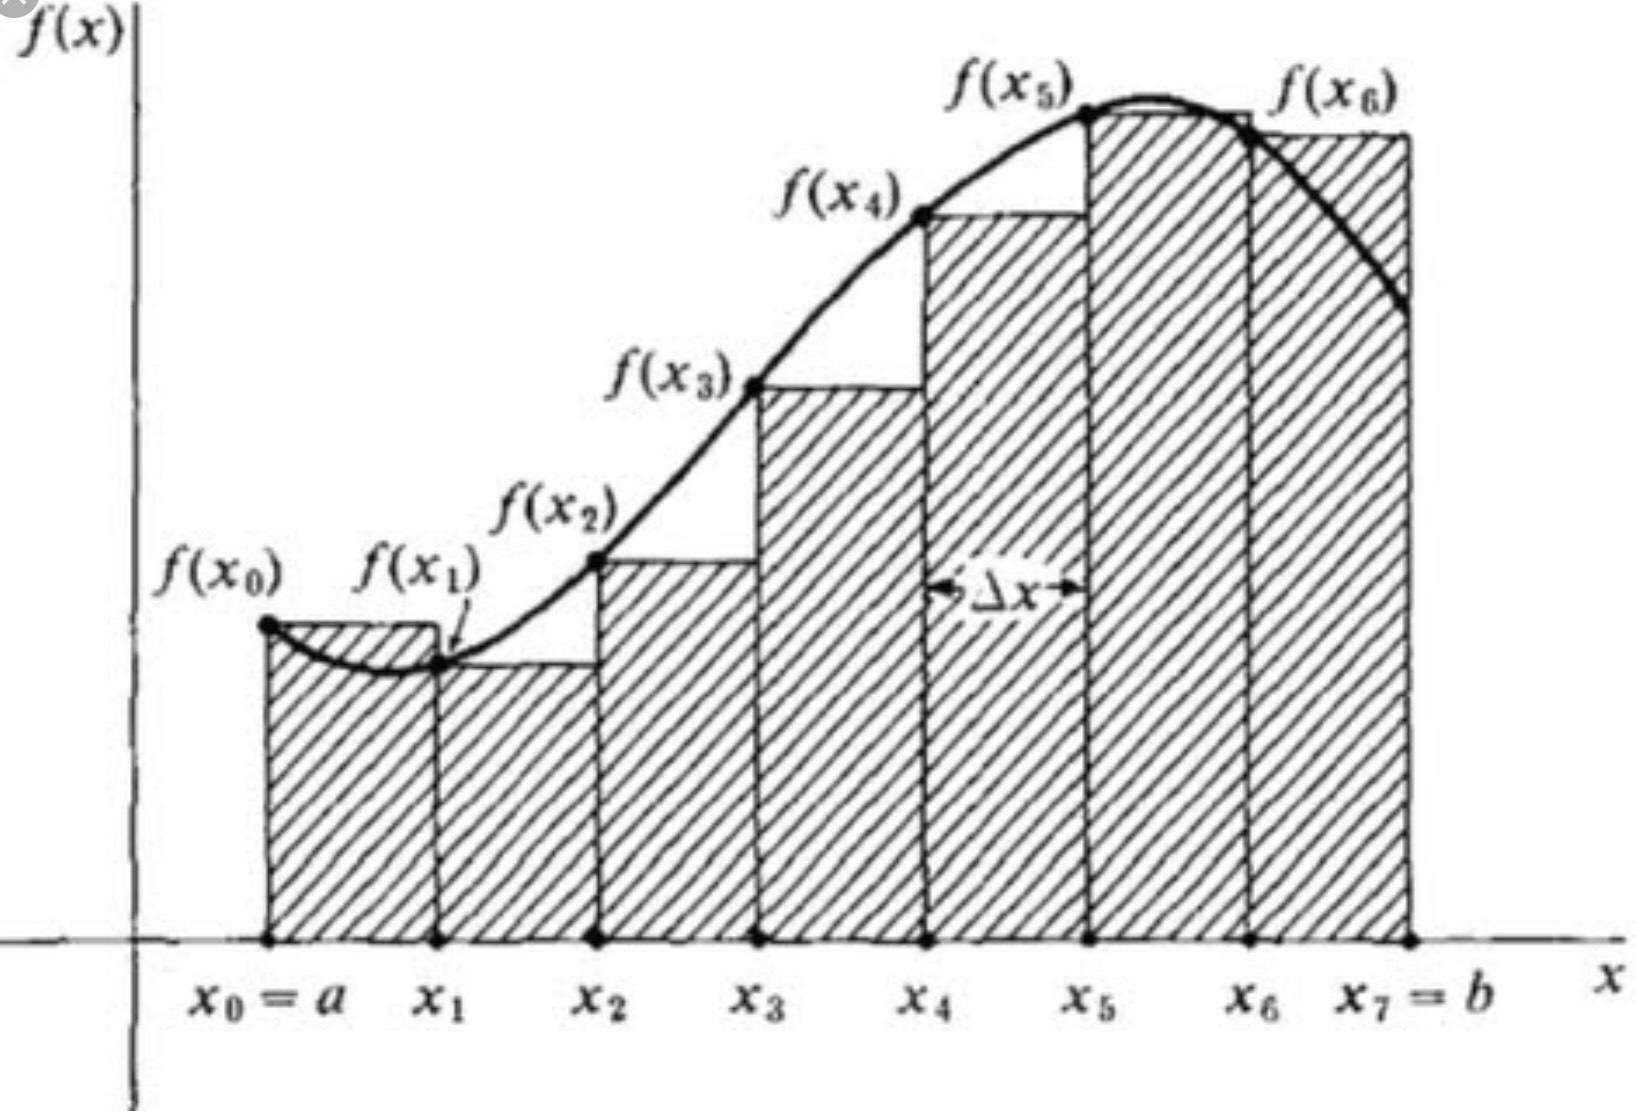
\includegraphics[width=\textwidth]{IMG_0380.jpg}
		\hspace*{10pt}\hbox{\thinspace{\tiny\itshape vias.org}}
		\caption{Single integration}
	\end{subfigure}% 
	~ 
	\begin{subfigure}{0.48\textwidth}
	
		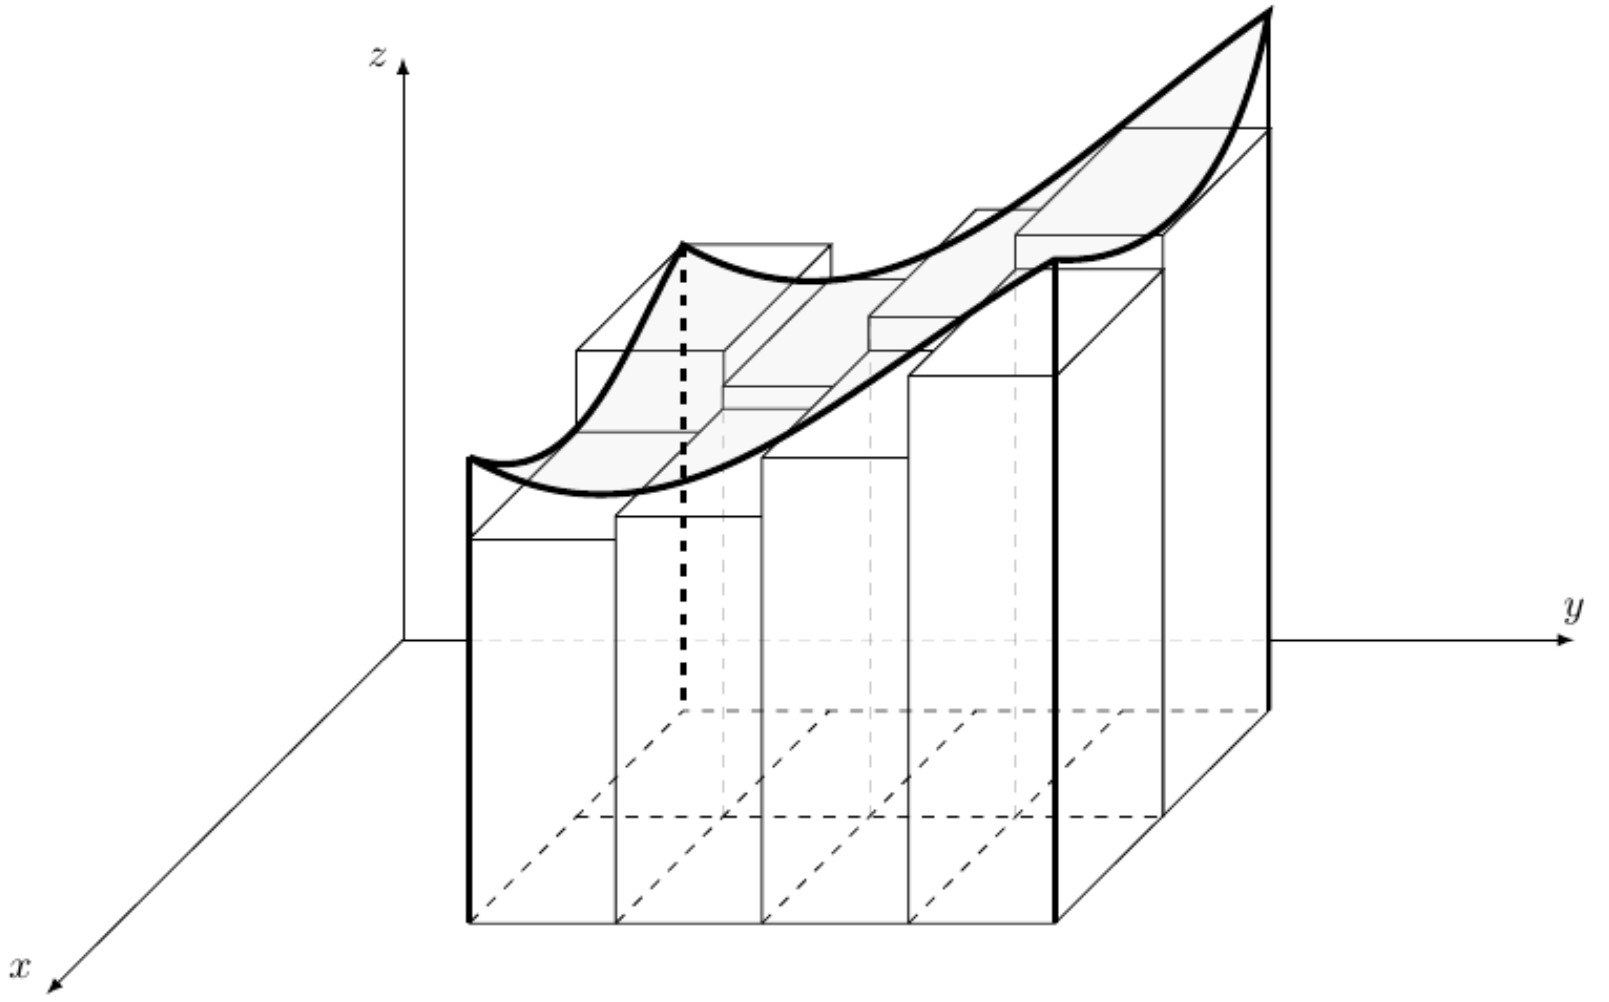
\includegraphics[width=\textwidth]{IMG_0385.jpg}
		\hspace*{10pt}\hbox{\thinspace{\tiny\itshape tex.stackexchange.com}}
		\caption{Double integration.}
		\label{fig:2}
	\end{subfigure}
\end{figure}

\end{frame}

\begin{frame}
\frametitle{\textbf{Riemann Double Integral}}
\begin{figure}
	\centering
	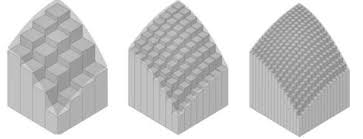
\includegraphics[width=.95\textwidth]{img_approx.jpg}
	\hspace*{10pt}\hbox{\thinspace{\tiny\itshape www.cis.umac.mo}}
\end{figure}
$$\iint\limits_{\mathbb{R}} f(x,y) dA = \lim\limits_{||\mathit{P}||\rightarrow 0} \sum_{i=1}^m \sum_{j=1}^n f(x_i^*,y_j^*)\Delta A_{i,j}$$
\end{frame}

\begin{frame}
\frametitle{\textbf{Properties}}
\begin{itemize}
	\item[(a)] $\iint\limits_{\mathbb{R}} c f(x,y) dx\,dy = c \iint\limits_{\mathbb{R}} f(x,y)dx\,dy$ if $c$ is a real number
	\item[(b)] $\iint\limits_{\mathbb{R}} [f(x,y) + g(x,y)] dx \,dy = \iint\limits_{\mathbb{R}} f(x,y)dx\,dy + \iint\limits_{\mathbb{R}} g(x,y)dx\,dy$
	\item[(c)] If $\mathbb{R}$ is the union of two nonoverlapping regions $\mathbb{R}_1 + \mathbb{R}_2$,
	$$\iint\limits_{\mathbb{R}}f(x,y)dx\,dy = \iint\limits_{\mathbb{R}_1}f(x,y)dx\,dy + \iint\limits_{\mathbb{R}_2}f(x,y)dx\,dy$$
	\item[(d)] If $f(x,y) \geq 0$ throughout $\mathbb{R}$, then $\iint\limits_{\mathbb{R}} f(x,y)dx\,dy \geq 0$
\end{itemize}
\end{frame}

\begin{frame}
\frametitle{\textbf{Evaluation of the Double Integral: Iterated Integral}}
It is generally impossible to evaluate the double integral using the definition. Instead it is typical to express the double integral as an iterated integral and evaluate as two single integrals.
$$\int_a^b \int_c^d f(x,y)dx\,dy = \int_a^b \Bigg[\int_c^d f(x,y)dx\Bigg]dy$$
\vspace{12pt}
\textbf{Examples:}
\begin{itemize}
	\item [(a)] $\int_1^4 \int_{-1}^2 (2x+6x^2y)dy\,dx$
	\item[(b)] $\int_{-1}^2 \int_1^4  (2x+6x^2y)dx\,dy$
\end{itemize}
\end{frame}

\begin{frame}
\frametitle{\textbf{Evaluation of the Double Integral: Fubini's Theorem}}

\begin{theorem}[Fubini's Theorem]
	If $f$ is a continuous function on rectangle $\mathbb{R} = \{(x,y)|a\leq b, c\leq d \}$ then
	$$\iint\limits_{\mathbb{R}} f(x,y)dA = \int_a^b \int_c^d f(x,y)dx\,dy = \int_c^d \int_a^b  f(x,y)dy\,dx $$
\end{theorem}


\vspace{12pt}

\textbf{Example:}

\begin{itemize}
	\item[(a)] Integrate $f(x,y) = 4xy$ on the rectangle with corners at $(0,0)$, $(4,0)$, $(0,2)$, and $(4,2)$.
\end{itemize}
\end{frame}

\begin{frame}
\frametitle{\textbf{Evaluation of the Double Integral: Factorizable $f$}}
If $f(x,y) = g(x)h(y)$ on $\mathbb{R} = [a,b] \times [c,d]$ then
$$\int_c^d \int_a^b f(x,y) dx\,dy = \int_a^bg(x)dx \int_c^d h(y)dy$$
Note: This only works if the limits are constant. (Don't depend on $x$ or $y$.)
\vspace{12pt}

\textbf{Example:}
\begin{itemize}
	\item[(a)] $\int_0^{\pi/2} \int_0^{\pi/2} \sin(x) \cos(y) dx \,dy$
\end{itemize}
\end{frame}

\begin{frame}
\frametitle{\textbf{Triple Integral}}
\begin{figure}
	\centering
	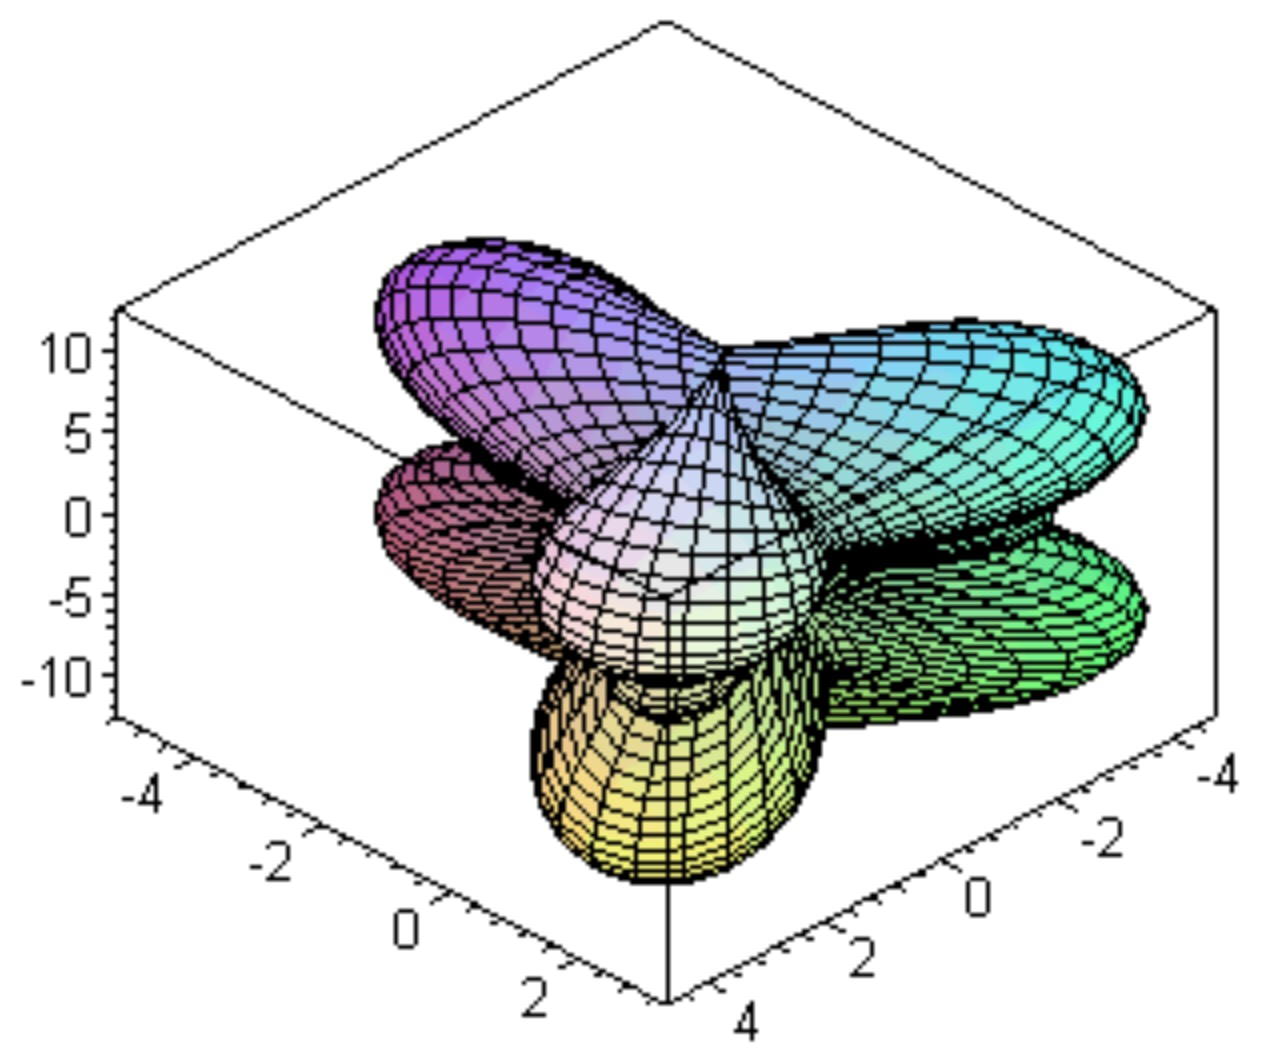
\includegraphics[height=.45\textheight]{IMG_0384.jpg}\\
	\hspace*{10pt}\hbox{\thinspace{\tiny\itshape maplesoft.com}}
\end{figure}

$$\iiint\limits_{\mathbb{R}} F(x,y,z) dV = \int_{x=a}^{x=b} \int_{y=y_1(x)}^{y=y_2(x)} \int_{z=z_1(x,y)}^{z=z_2(x,y)} F(x,y,z) dz\,dy\,dx$$
\textbf{Example:}
\begin{itemize}
	\item[(a)] $\int_0^1 \int_0^{1-x} \int_0^{2-x} xyz \,dz\,dy\,dx$
\end{itemize}
\end{frame}

\end{document}
